\documentclass[fleqn]{article}
\usepackage{graphicx}
\usepackage{subcaption}
\usepackage{amsmath}
\usepackage{amssymb}
\usepackage{bm}
\usepackage{pgfplots}
\pgfplotsset{compat=1.18}
\usepackage[margin=25truemm]{geometry}
\usepackage{hyperref}

\title{CSCI2750 Homework 4}
\author{Wong Cheuk Yin 1155192671}
\date{\today}

\begin{document}
    \maketitle
    \section{Problem 1}

    \textbf{Given the following dataset:}

    \medskip

    \begin{tabular}{c|c|c}
        \hline
        $i$ & $x^{(i)}$ & label \\
        \hline
        1 & $(-3, 2, 0)$ & $+$ \\
        2 & $(-2, -2, 1)$ & $-$ \\
        3 & $(-1, -1, -1)$ & $-$ \\
        4 & $(0, 0, 1)$ & $-$ \\
        5 & $(1, -2, -1)$ & $-$ \\
        6 & $(2, 1, 2)$ & $+$ \\
        7 & $(3, -1, 0)$ & $+$ \\
        \hline
    \end{tabular}
    
    \medskip
    \noindent We use the GINI index to determine the best split point.

    \medskip
    \noindent At the root ($7$ points: $3$ positive, $4$ negative), checking candidate threshold splits gives a minimum weighted Gini of $\frac{8}{35}\approx 0.2286$, achieved by $x_1\le 1$ and tied with a split on $x_2\le 0$. We choose
    \[
    x_1\le 1.
    \]
    Then:
    \begin{itemize}
        \item Right child ($x_1>1$): $\{x^{(6)},x^{(7)}\}$, both $+$, hence pure leaf ($+$).
        \item Left child ($x_1\le 1$): $\{x^{(1)},x^{(2)},x^{(3)},x^{(4)},x^{(5)}\}$ with labels $(+,-,-,-,-)$.
    \end{itemize}

    \noindent Split the left child by
    \[
    x_1\le -3,
    \]
    so that:
    \begin{itemize}
        \item Left leaf: $\{x^{(1)}\}$, pure $+$.
        \item Right leaf: $\{x^{(2)},x^{(3)},x^{(4)},x^{(5)}\}$, pure $-$.
    \end{itemize}

    \noindent Therefore, a 5-node decision tree is:
    \begin{itemize}
        \item If $x_1>1$, predict $+$;
        \item else if $x_1\le -3$, predict $+$;
        \item else predict $-$.
    \end{itemize}
    \noindent This tree has 2 internal nodes and 3 leaves (total 5 nodes), and it classifies all training points correctly.

    \[
    \text{Training error}=\frac{0}{7}=0.
    \]

    \newpage
    \section{Problem 2}
    \textbf{Given the following dataset:}
    \[
    \textbf{a} = (0,1,2,1), \quad \textbf{b} = (2,3,4,2), \quad \textbf{c} = (-2,-1,1,3), \quad \textbf{d} = (1,0,1,0), \quad \textbf{e} = (3,4,5,3).
    \]

    \noindent Initially, we have 5 clusters: $C_1=\{a\}, C_2=\{b\}, C_3=\{c\}, C_4=\{d\}, C_5=\{e\}$.

    \noindent Pairwise Manhattan distances:
    \[
    \begin{aligned}
    &d(a,b)=7,\ d(a,c)=7,\ d(a,d)=4,\ d(a,e)=11,\\
    &d(b,c)=12,\ d(b,d)=9,\ d(b,e)=4,\\
    &d(c,d)=7,\ d(c,e)=14,\ d(d,e)=13.
    \end{aligned}
    \]

    \noindent Hence, the dissimilarity matrix (in the order $C_1, C_2, C_3, C_4, C_5$) is
    \[
    D=
    \begin{bmatrix}
    0 & 7 & 7 & 4 & 11\\
    7 & 0 & 12 & 9 & 4\\
    7 & 12 & 0 & 7 & 14\\
    4 & 9 & 7 & 0 & 13\\
    11 & 4 & 14 & 13 & 0
    \end{bmatrix}.
    \]

    \noindent Observe that minimum Manhattan distance in the matrix is $d(a,d)=4$ and $d(b,e)=4$,

    \medskip
    First merge: $C_4$ into $C_1$ 

    Second merge: $C_5$ into $C_2$.

    \medskip
    \noindent New clusters: $C_1=\{a,d\}, C_2=\{b,e\}, C_3=\{c\}$.

    \noindent New dissimilarity matrix (in the order $C_1, C_2, C_3$):
    \[
    D=
    \begin{bmatrix}
    0 & 7 & 7\\
    7 & 0 & 12\\
    7 & 12 & 0
    \end{bmatrix}.
    \]

    \noindent Observe that minimum Manhattan distance in the matrix is $d(C_1, C_3)=7$ and $d(C_1, C_2)=7$.

    \medskip
    Third merge(arbitrarily chosen since tied): $C_3$ into $C_1$ 

    \medskip
    \noindent New clusters: $C_1=\{a,c,d\}$, $C_2=\{b,e\}$. (The result clusters for K=2)
    
    \medskip
    \noindent Then we merge $C_1$ and $C_2$ into $C_1$(because dendogram is a tree, which means K=1) and get the final clusters: $C_1=\{a,c,d,b,e\}$.

    \begin{figure}[htbp]
        \centering
        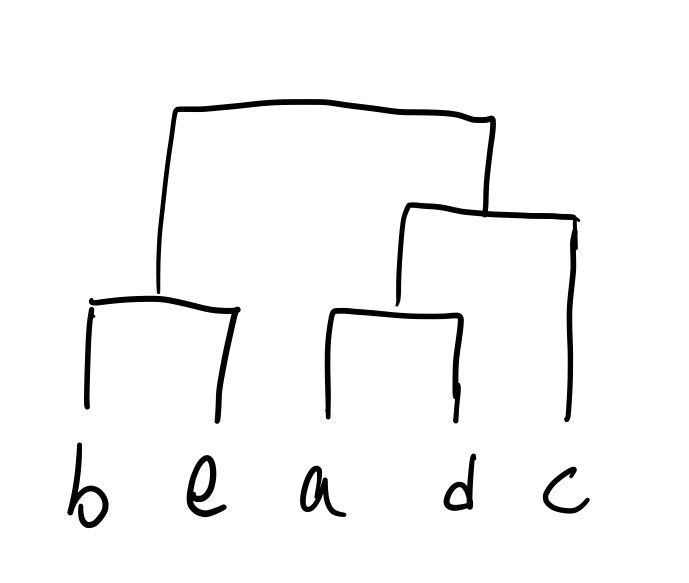
\includegraphics[width=0.4\linewidth]{dendo.jpeg}
        \caption{Resultant Dendrogram.}
    \end{figure}

    \newpage
    \section{Problem 3}

    \noindent Given
    \[
    \mathcal{D}=\{x^{(i)}\mid x^{(i)}=2i,\ i=1,\ldots,m\}.
    \]

    \subsection*{(a) Case $m=6$, initial center $z_1=x^{(1)}$, and $K=3$}
    \noindent Data points:
    \[
    \mathcal{D}=\{2,4,8,16,32,64\}.
    \]

    \noindent \textbf{K-centers iterations:}
    \begin{itemize}
        \item Given inital center: $z_1 = 2$
        \item Step 1: choose $z_2 = 64$  (farthest point from $z_1$).
        \item Step 2: choose $z_3 = 32$ (farthest point from $z_1$ and $z_2$).
    \end{itemize}

    \noindent Final centers:
    \[
    z_1 = 2,\quad
    z_2 = 64,\quad
    z_3 = 32.
    \]

    \noindent Resultant clusters (by nearest-center assignment):
    \[
    Z_1=\{2,4,8,16\},\quad
    Z_2=\{64\},\quad
    Z_3=\{32\}.
    \]

    \noindent Radius of clustering:
    \[
    \mathcal{R}(Z)=\max_{x\in \mathcal{D}}\min_{k\in\{1,2\}}|x-z_k|
    =16-2=14.
    \]

    \subsection*{(b) Compute SSE and BSS for the clustering result in (a)}

    \noindent Mean of each cluster:
    \[
    \mu_1 = \frac{2+4+8+16}{4} = 7.5,\quad
    \mu_2 = 64,\quad
    \mu_3 = 32.
    \]

    \noindent SSE:
    \[
    \sum_{k=1}^{3}\sum_{x\in Z_k}(x-\mu_k)^2
    =((2-7.5)^2+(4-7.5)^2+(8-7.5)^2+(16-7.5)^2) +(64-64)^2+(32-32)^2
    =115
    \]

    \noindent Global mean:
    \[
    \bar{x} = \frac{2+4+8+16+64+32}{6} = 16.
    \]

    
    \noindent BSS:
    \[
    \sum_{k=1}^{3}|Z_k|(\mu_k-\bar{x})^2
    =4\cdot(7.5-16)^2 + 1\cdot(64-16)^2 + 1\cdot(32-16)^2
    \]

    \newpage
    \subsection*{(c) Proof for $\mathcal{R}(Z)\le 2^{m-1}$ for K=2}
    \noindent With no fixed initial center, $z_1$ will be chosen randomly from the dataset.

    \medskip
    \noindent If $z_1 = 2^{i}$ for some $i\in\{1,2,\ldots,m-1\}$, $z_2$ will always be $2^{m}$ since it must be the farthest point from $z_1$. In this case, all remaining points will be assigned to $Z_1$ because they are all closer to $z_1$ than to $z_2$. Hence, we have:
    \[
        Z_1=\{2, 4, 8, \ldots, 2^{m-1}\},\quad
        Z_2=\{2^{m}\},\quad
    \]
    To get the greatest possible radius, $z_1$ should be $2$ or $2^{m-1}$ since the distance between $2$ and $2^{m-1}$ is the greatest.
    \[
    \mathcal{R}(Z)=\max_{x\in \mathcal{D}}\min_{k\in\{1,2\}}|x-z_k|
    =2^{m}-2^{m-1}=2^{m-1}.
    \]
    
    \noindent Case 2, If $z_1 = 2^{m}$, $z_2$ will always be $2$ since it must be the farthest point from $z_1$. In this case, all remaining points will be assigned to $Z_2$ because they are all closer to $z_2$ than to $z_1$. Hence, we have:
    \[
    Z_1=\{2^{m}\},\quad
    Z_2=\{2, 4, 8, \ldots, 2^{m-1}\},\quad
    \]
    To get the greatest possible radius, $z_1$ should be $2^{m}$ since the distance between $2^{m}$ and $2$ is the greatest.
    \[
    \mathcal{R}(Z)=\max_{x\in \mathcal{D}}\min_{k\in\{1,2\}}|x-z_k|
    =2^{m}-2=2^{m-1}.
    \]

    \noindent We can see, there is no case that can get a radius greater than $2^{m-1}$, Therefore,
    \[
    \mathcal{R}(Z)\le 2^{m-1}.
    \]

    \section{Problem 4}
    \subsection{(a) Set of unique items}
    \[
    \mathcal{I} = \{\text{Phone Charger}, \text{Passport}, \text{Water Bottle}, \text{Power Bank}\}.
    \]

    \subsection{(b) Apriori algorithm}
    \noindent There are $7$ transactions, so
    \[
    \mathrm{supp}(X)=\frac{\#\{\text{transactions containing }X\}}{7}.
    \]
    With $\mathrm{minsup}=0.7$, an itemset must appear at least $5$ times to be frequent.

    \medskip
    \noindent \textbf{All itemsets and supports}
    \[
    \begin{array}{c|c|c}
        \hline
        \text{Itemset } X & \mathrm{supp}(X) & \text{Frequent?} \\
        \hline
        \{\text{Phone Charger}\} & 6/7 & \text{Yes} \\
        \{\text{Passport}\} & 4/7 & \text{No} \\
        \{\text{Water Bottle}\} & 6/7 & \text{Yes} \\
        \{\text{Power Bank}\} & 3/7 & \text{No} \\
        \hline
        \{\text{Phone Charger},\text{Passport}\} & 3/7 & \text{No} \\
        \{\text{Phone Charger},\text{Water Bottle}\} & 5/7 & \text{Yes} \\
        \{\text{Phone Charger},\text{Power Bank}\} & 3/7 & \text{No} \\
        \{\text{Passport},\text{Water Bottle}\} & 3/7 & \text{No} \\
        \{\text{Passport},\text{Power Bank}\} & 1/7 & \text{No} \\
        \{\text{Water Bottle},\text{Power Bank}\} & 3/7 & \text{No} \\
        \hline
        \{\text{Phone Charger},\text{Passport},\text{Water Bottle}\} & 2/7 & \text{No} \\
        \{\text{Phone Charger},\text{Passport},\text{Power Bank}\} & 1/7 & \text{No} \\
        \{\text{Phone Charger},\text{Water Bottle},\text{Power Bank}\} & 3/7 & \text{No} \\
        \{\text{Passport},\text{Water Bottle},\text{Power Bank}\} & 1/7 & \text{No} \\
        \hline
        \{\text{Phone Charger},\text{Passport},\text{Water Bottle},\text{Power Bank}\} & 1/7 & \text{No} \\
        \hline
    \end{array}
    \]

    \noindent Therefore, the frequent itemsets (Apriori output) are
    \[
    \mathcal{I}^{(1)}=\big\{\{\text{Phone Charger}\},\{\text{Water Bottle}\}\big\},\quad
    \mathcal{I}^{(2)}=\big\{\{\text{Phone Charger},\text{Water Bottle}\}\big\}
    \]
    \subsection{(c) Strong association rules}
    \noindent Since $\mathrm{minconf}=0.8$, the strong rules from
    $\{\text{Phone Charger},\text{Water Bottle}\}$ are:
    \[
    \{\text{Phone Charger}\}\Rightarrow\{\text{Water Bottle}\},
    \quad
    \mathrm{conf}
    =\frac{\mathrm{supp}(\{\text{Phone Charger},\text{Water Bottle}\})}
    {\mathrm{supp}(\{\text{Phone Charger}\})}
    =\frac{5/7}{6/7}
    =\frac{5}{6}\approx 0.833.
    \]
    \[
    \{\text{Water Bottle}\}\Rightarrow\{\text{Phone Charger}\},
    \quad
    \mathrm{conf}
    =\frac{\mathrm{supp}(\{\text{Phone Charger},\text{Water Bottle}\})}
    {\mathrm{supp}(\{\text{Water Bottle}\})}
    =\frac{5/7}{6/7}
    =\frac{5}{6}\approx 0.833.
    \]

    \subsection{(d) Recommendation for Aaron}
    \noindent Recommend \textbf{Water Bottle}. Aaron already has Phone Charger; the strong rule
    $\{\text{Phone Charger}\}\Rightarrow\{\text{Water Bottle}\}$ is a strong association rule, so among people who pack a phone charger, a water bottle is a highly associated next item, and Aaron did not list it.

    \subsection{(e) Recommendation for Hannah}
    \noindent Recommend \textbf{Phone Charger}. Hannah already has Water Bottle; the strong rule
    $\{\text{Water Bottle}\}\Rightarrow\{\text{Phone Charger}\}$ is a strong association rule, so among people who pack a water bottle, a phone charger is a highly associated next item, and Hannah did not list it.

    \section{Problem 5}
    \subsection{(a) Study of MATLAB SVD implementation}
    For image preprocessing, the given code did:
    \begin{itemize}
        \item Convert the image to grayscale (\texttt{rgb2gray}).
        \item Cast pixel values to \texttt{double} because the build-in svd function requires double.
        \item Normalize intensities by dividing by $\max(X(:))$, so entries lie in $[0,1]$.
    \end{itemize}

    \medskip
    \noindent Then, function svd() was called to compute the corresponding U, S, V, which comes as single vector.
    To get the full matrices, we need to reshape the vectors back into the original dimensions by the following code:
    \begin{verbatim}
        U_new = U(:, 1:k);
        S_new = diag(S);
        S_new = diag(S_new(1:k));
        V_new = V(:,1:k);
    \end{verbatim}

    \begin{itemize}
        \item U is duplicated to every row of the matrix to get $\bar{U}$.
        \item Let the i-th diagonal element of $\bar{\Sigma}$, the i-th element of the S. Other elements are set to 0. 
        \item V is duplicated to every column of the matrix to get $\bar{V}$.
    \end{itemize}

    Finally, we can reconstruct the image by $X = \bar{U} \bar{\Sigma} \bar{V}'$ which is implemented in the following code:
    \begin{verbatim}
        X_new = U_new * S_new * V_new';
    \end{verbatim}

    \newpage
    \subsection{(b) SVD compression on a chosen image}
    Chosen image:
    \begin{figure}[htbp]
        \centering
        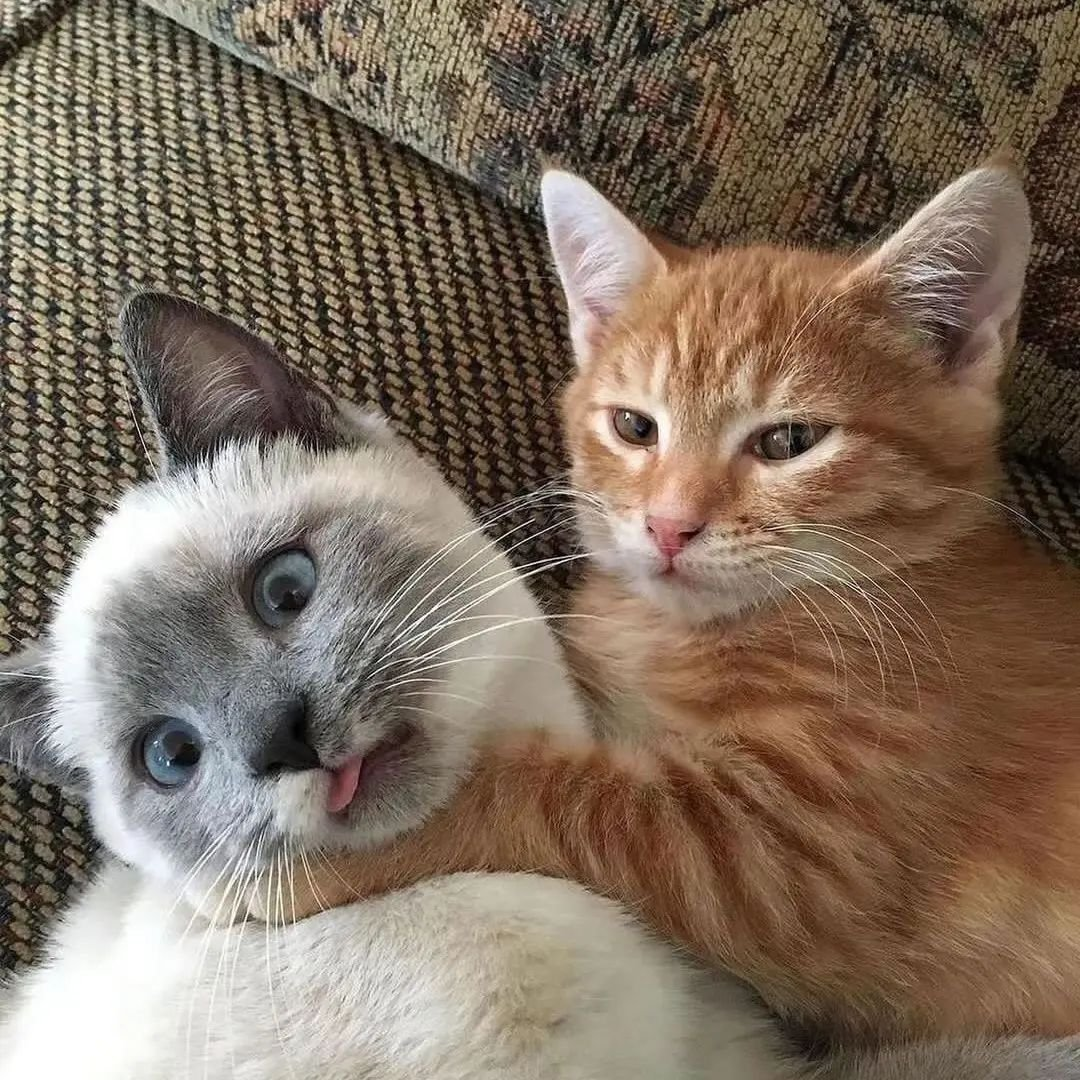
\includegraphics[width=0.3\linewidth]{orangecat.jpeg}
        \caption{An evil orange cat(right) attempting to execute a Siamese cat(left) by shutting down his respiratory system forever. I hope he survives. :(}
    \end{figure}
    
    \noindent The image's resolution is $1080\times 1080$, which means:
    \[
    m = 1080, \quad n = 1080.
    \]

    \noindent We need to follow the rule below to make the compression meaningful:
    \[
    k < \frac{mn}{m+n+1} = \frac{1080\times 1080}{1080+1080+1} \approx 539.75.
    \]

    \noindent we choose $k = 200$ and compute the the compressed image with MATLAB code implemented with the logic in (a).
    \begin{figure}[htbp]
        \centering
        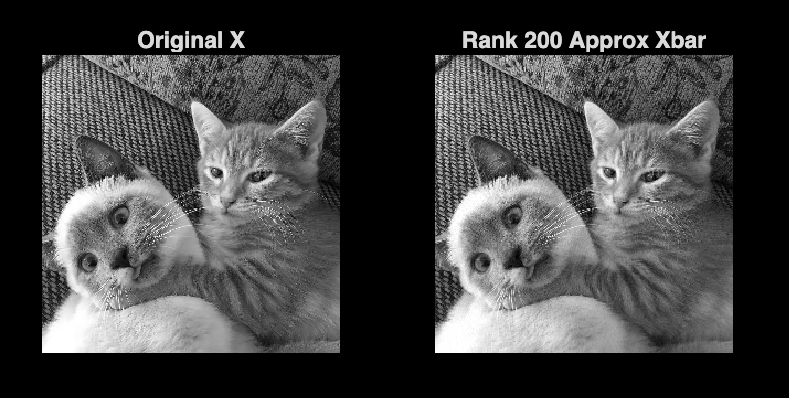
\includegraphics[width=0.6\linewidth]{svdcat.png}
        \caption{Visualisation of \textbf{$X$} and its rank-200 approximation \textbf{$\bar{X}$}.}
    \end{figure}

    \noindent Apparently, the quality did not drops significantly. The cat is still recognizable.

    \newpage
    \subsection{(c) Compression with different compression rates}
    We can obtain $k$ needed to achieve the desired compression rate by the following formula:

    \[
    \text{Compression rate} = \frac{\mathrm{storage}(\bar{X})}{\mathrm{storage}(X)} = \frac{k(m+n+1)}{mn} = \frac{k \times (1080+1080+1)}{1080\times 1080}
    \]

    \[
    k = \frac{1080^{2}}{2161} \times \text{Compression rate}
    \]

    \noindent We can obtain the following table:

    \medskip
    \begin{tabular}{c|c}
        \hline
        \text{Compression rate} & \text{Required rank $k$ (closest integer)} \\
        \hline
        10\% & 54\\
        20\% & 108 \\
        40\% & 216 \\
        80\% & 432 \\
        \hline
    \end{tabular}

    \medskip
    \noindent Visualisation by MATLAB code:
    \begin{figure}[htbp]
        \centering
        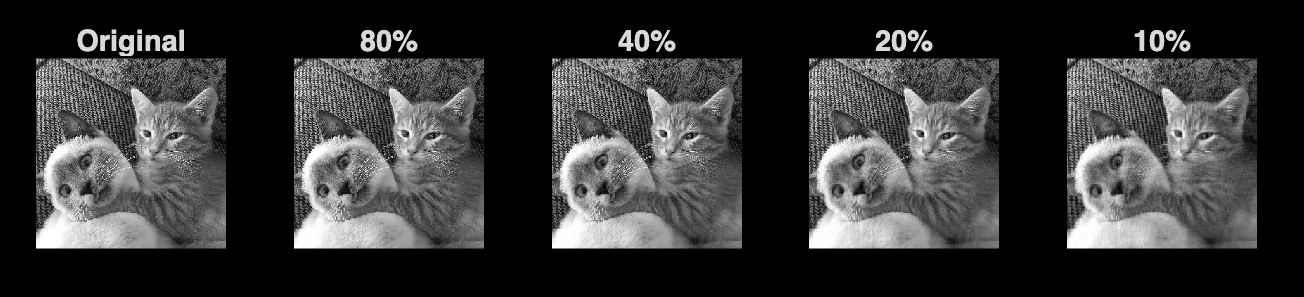
\includegraphics[width=1\linewidth]{different_rate.png}
        \caption{Visualisation of the compressed images with different compression rates.}
    \end{figure}

    \subsection{(d) SVD for RGB image}
    Skip the X = rgb2gray in order to keep the original RBG image. We can compute the SVD with the following code:
    \begin{verbatim}
        k = 200;  %change if needed
        X = imread('orangecat.jpeg'); 
        X = double(X);
        X = X ./ max(X(:));

        R = X(:, :, 1);
        G = X(:, :, 2);
        B = X(:, :, 3);
        [Ur, Sr, Vr] = svd(R);
        [Ug, Sg, Vg] = svd(G);
        [Ub, Sb, Vb] = svd(B);

        Rbar = Ur(:,1:k) * Sr(1:k,1:k) * Vr(:,1:k)';
        Gbar = Ug(:,1:k) * Sg(1:k,1:k) * Vg(:,1:k)';
        Bbar = Ub(:,1:k) * Sb(1:k,1:k) * Vb(:,1:k)';
        
        Xbar = cat(3, Rbar, Gbar, Bbar);
        
        figure;
        subplot(1, 2, 1);
        imshow(X);
        title('Original RGB');
        subplot(1, 2, 2);
        imshow(Xbar);
        title(sprintf('RGB per-channel rank-%d SVD', k));
    \end{verbatim}

    \begin{figure}[htbp]
        \centering
        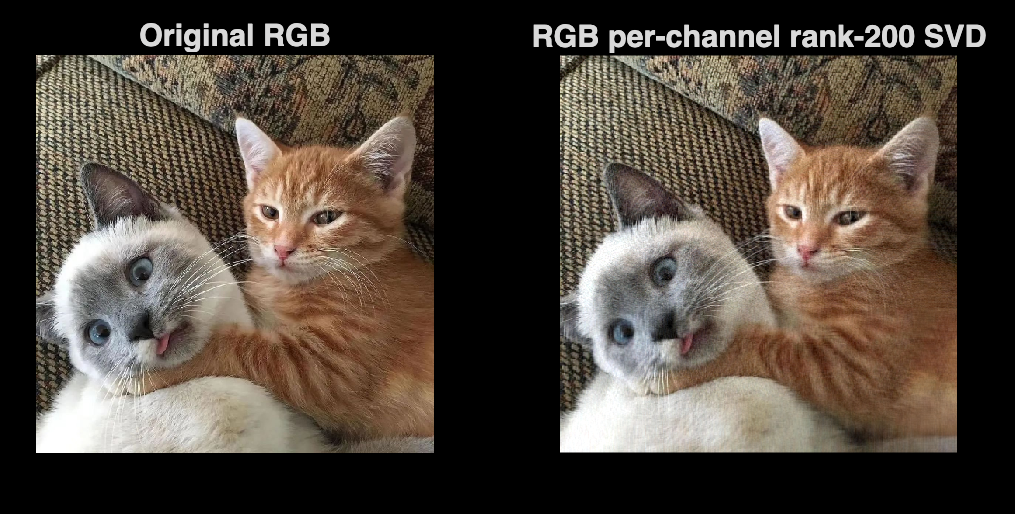
\includegraphics[width=0.6\linewidth]{rgb_svd_compare.png}
        \caption{Visualisation of the original RGB image and its rank-200 approximation.}
    \end{figure}

    \noindent The quality is still good. The cat is still recognizable.

\end{document}